\documentclass[a4paper,12pt]{article}
\usepackage[T2A]{fontenc}
\usepackage[utf8x]{inputenc}
\usepackage[english,russian]{babel}
\usepackage{amssymb,amsfonts,amsmath,mathtext}
\usepackage[unicode]{hyperref}
\usepackage{listings}
\usepackage{graphicx}
\graphicspath{{images/}}
\newcommand{\anonsection}[1]{\section*{#1}\addcontentsline{toc}{section}{#1}}

\begin{document}

% Титульный лист

\begin{titlepage}
\newpage

\begin{center}

\textit{Министерство науки и высшего образования Российской Федерации \\ 
Федеральное государственное бюджетное образовательное \\
учреждение высшего образования \\
«Московский государственный технический университет \\
имени Н.Э. Баумана (национальный исследовательский университет)» \\
(МГТУ им. Н.Э. Баумана) \\}
\hrulefill
\end{center}

\vspace{2em}

\begin{flushleft}
ФАКУЛЬТЕТ <<Информатика и системы управления>> \\
\vspace{0.5em}
КАФЕДРА <<Программное обеспечение ЭВМ и информационные технологии>>
\end{flushleft}


\vspace{8em}

\begin{center}
\LARGE Лабораторная работа №1 \\
\end{center}

\vspace{1.5em}

\begin{center}
\textsc{Расстояние Левенштейна}
\end{center}

\vspace{6em}

\begin{center}
Головнев Н.В.

\vspace{4em}

ИУ7-54Б
\end{center}

\vspace{\fill}

\begin{center}
Москва 2019
\end{center}

\end{titlepage}

\tableofcontents

% Введение

\newpage
\anonsection{ВВЕДЕНИЕ}

\begin{flushleft}
Цель данной лабораторной работы:\\
Изучить алгоритмы поиска редакционного расстояния Левенштейна (или Дамерау-Левенштейна) и реализовать эти алгоритмы. \\
Постановка задачи:\\
\begin{enumerate}
\item Реализовать обычный алгоритм поиска редакционного расстояния Левенштейна;
\item Реализовать рекурсивный алгоритм поиска редакционного расстояния Левенштейна;
\item Реализовать алгоритм поиска редакционного расстояния Дамерау-Левенштейна;
\end{enumerate}
\end{flushleft}

% Аналитическая часть

\newpage
\section{АНАЛИТИЧЕСКАЯ ЧАСТЬ}
\subsection{Описание алгоритмов}

Часто требуется измерить различие между двумя строками (например, в эволюционных, структуральных или функциональных исследованиях биологических строк, в хранении текстовых баз данных, в методах проверки правописания). Есть несколько способов формализации понятия расстояния между строками. Одна общая, и простая, формализация называется редакционным расстоянием; она основана на преобразовании (или редактировании) одной строки в другую серией операций редактирования, выполняемых над отдельными символами. Разрешенные операции редактирования - это \textit{вставка} (insertion) символа в первую строку, \textit{удаление} (deletion) символа из первой строки и \textit{подстановка} или \textit{замена} (substitution или replace) символа из первой строки символом из второй строки. \\
Пусть I - insert, \\
D - delete, \\
R - replace, \\
M - никакая операция. \\
Тогда строка \textit{vintner} может быть доредактирована до \textit{writers} следующим образом: \\
\begin{table}[h]
\begin{center}
\begin{tabular}{ccccccccc}
R & I & M & D & M & D & M & M & I \\
v & & i & n & t & n & e & r & \\
w & r & i & & t & & e & r & s \\
\end{tabular}
\end{center}
\end{table}
\\
\textbf{Определение.} Строка над алфавитом I, D, R, M, которая описывает преобразование одной строки в другую, называется \textit{редакционным предписанием} или, для краткости, \textit{предписанием} этих 2-х строк. \\
\\
\textbf{Определение}. \textit{Редакционное расстояние} между двумя строками определяется как минимальное число редакционных операций - вставок, удалений и подстановок, необходимое для преобразования первой строки во вторую[\ref{sources:source3}]. Совпадения операциями не сичитаются и не засчитываются. \\
\\
\textbf{Задача о редакционном расстоянии} - это задача о вычислении редакционного расстояния между 2-мя данными строками вместе с оптимальным  предписанием, описывающим преобразование, на котором этот минимум достигается. Оптимальное предписание - редакционное предписание, использующее минимальное число редакционных операций. \\
\\
\textbf{Определение.} Для 2-х строк, S$_1$ и S$_2$, значение \textit{D}(\textit{i}, \textit{j}) определяется как редакционное	расстояние между S$_1$[1..\textit{i}] и S$_2$[1..\textit{j}]. \\
\\
\textit{D}(\textit{i}, \textit{j}) - Рекуррентное соотношение. \\

\begin{equation}
D[i,j] = \left\{
\begin{array}{ll}
0, & i = 0, j = 0 \\
i, & j = 0, i > 0 \\
j, & j > 0, i < 0 \\
min\left\{
\begin{array}{ll}
D(i,j - 1) + 1, \\
D(i - 1,j) + 1, \\
D(i - 1,j - 1) + t(S_1[i],S_2[j])
\end{array}
\right.
& j > 0, i > 0
\end{array}
\right.
\end{equation}
\\
где

\begin{equation}
t(S_1[i],S_2[j]) = \left\{
\begin{array}{ll}
0, & S_1[i] = S_2[j] \\
1 & \text{otherwise}
\end{array}
\right.
\end{equation}

Исследования Ф. Дамерау показали, что наиболее частая ошибка при наборе слова – перестановка двух соседних букв, транспозиция T (transposition)[\ref{sources:source2}]. \\
При использовании расстояния Дамерау   –   Левенштейна за единичное расстояние принимают следующие действия: I (insert) – добавление символа;  D  (delete) – удаление символа;  R  (replace) – замена символа;  T  (transposition) – перестановка двух соседних символов.  \\

Расстояние Дамерау-Левенштейна между 2-мя строками $S_1$ и $S_2$ определяется функцией $D(|S_1|,|S_2|))$, равной:
\begin{equation}
D(i,j) = \left\{
\begin{array}{ll}
max(i,j) & if min(i,j) = 0, \\
min\left\{
\begin{array}{l}
D(i-1,j)+1\\
D(i,j-1)+1\\
D(i-1,j-1) + t(S_1[i],S_2[j])\\
D(i-2,j-2) + 1\\
\end{array}
\right. & if i,j>1 and S_1[i]=S_2[j-1] \linebreak and S_1[i-1]=S_2[j], \\
min\left\{
\begin{array}{l}
D(i-1,j)+1\\
D(i,j-1)+1\\
D(i-1,j-1) + t(S_1[i],S_2[j])\\
\end{array}
\right. & otherwise \\
\end{array}
\right.
\end{equation}

\subsection{Вывод}
% Сделай эту каку
% Конструкторская часть

\newpage
\section{КОНСТРУКТОРСКАЯ ЧАСТЬ}

\subsection{Разработка алгоритмов}

На вход у всех алгоритмов передаются в качестве параметров:
\begin{enumerate}
\item Адреса строк;
\item Длины строк (не должны быть равны 0);
\item Адрес переменной, в которой будет храниться результат;
\item Область памяти (для стандартных реализаций поиска редакционного расстояния), в которой сохраняется матрица с редакционными расстояниями.
\end{enumerate}
Возвращаемое значение: код ошибки (0 в случае успеха, иначе отрицательное значение). \\
Побочные эффекты: изменяются значения в матрице и в переменной результата.

\newpage
\subsection{Схемы алгоритмов}

%Добавить сюда картинки из yEd

\begin{figure}[h!]
\center{\includegraphics[scale=0.25]{levenstein.png}}
\caption{Схема стандартного алгоритма Левенштейна (Начало)}
\label{images:levenstein}
\end{figure}

\begin{figure}[p]
\center{\includegraphics[scale=0.25]{levenstein2.png}}
\caption{Схема стандартного алгоритма Левенштейна (Конец)}
\label{images:levenstein2}
\end{figure}

\begin{figure}[p]
\center{\includegraphics[scale=0.25]{recursive_levenstein.png}}
\caption{Схема рекурсивного алгоритма Левенштейна (Начало)}
\label{images:recursive_levenstein}
\end{figure}

\begin{figure}[p]
\center{\includegraphics[scale=0.25]{recursive_levenstein2.png}}
\caption{Схема рекурсивный алгоритма Левенштейна (Конец)}
\label{images:recursive_levenstein2}
\end{figure}

\begin{figure}[p]
\center{\includegraphics[scale=0.25]{damerlau.png}}
\caption{Схема стандартного алгоритма Дамерау-Левенштейна (Начало)}
\label{images:damerau_levenstein}
\end{figure}

\begin{figure}[p]
\center{\includegraphics[scale=0.25]{damerlau2.png}}
\caption{Схема стандартного алгоритма Дамерау-Левенштейна (Конец)}
\label{images:damerau_levenstein2}
\end{figure}

\newpage
\subsection{Вывод}


\newpage
\section{ТЕХНОЛОГИЧЕСКАЯ ЧАСТЬ}
\subsection{Требования к программному обеспечению}

\begin{flushleft}
Программа должна работать на операционной системе Arch Linux. Программа должна
содержать 2 режима:
\begin{itemize}
\item Пользовательский
\item Экспериментальный
\end{itemize}
В пользовательском режиме пользователь должен иметь возможность вводить строки и получать результат работы 3-х алгоритмов. В экспериментальном режиме засекается процессорное время работы каждого алгоритма, результаты записываются в отдельные файлы. Впоследствии данные из этих файлов можно вывести в виде графика.
\end{flushleft}

\newpage
\subsection{Средства реализации}
Для реализации данных алгоритмов был выбран язык программирования С, компилятор
gcc и некоторые функции из библиотеки glibc (memcpy, malloc и тд...). \\
Удобства, предоставляемые языком C:
\begin{itemize}
\item Прямой доступ к памяти;
\item Возможность составлять простейшие структуры данных;
\end{itemize}
Для вывода графиков использовался Python3 (библиотека Matplotlib)

\newpage
\subsection{Листинг кода}
\lstdefinestyle{customc}{
  belowcaptionskip=1\baselineskip,
  breaklines=true,
  frame=L,
  xleftmargin=\parindent,
  language=C,
  showstringspaces=false,
  basicstyle=\footnotesize\ttfamily
}

\lstinputlisting[captionpos=b, caption=\label{listings:listing1}Стандартная реализация алгоритма Левенштейна(\ref{images:levenstein}), style=customc]{listing1.c}
\lstinputlisting[captionpos=b, caption=\label{listings:listing2}Рекурсивная реализация алгоритма Левенштейна(\ref{images:recursive_levenstein}), style=customc]{listing2.c}
\lstinputlisting[captionpos=b, caption=\label{listings:listing3}Стандартная реализация алгоритма Дамерау-Левенштейна(\ref{images:damerau_levenstein}), style=customc]{listing3.c}

\newpage
\subsection{Вывод}

\newpage
\section{ЭКСПЕРИМЕНТАЛЬНАЯ ЧАСТЬ}
\subsection{Характеристики аппаратного и программного обеспечения}
\flushleft{Тестирование приложения проводилось на машине со следующими характеристиками:\\}
\begin{itemize}
\item Процессор Intel® Core™ i7-7700HQ;
\item Оперативная память 16 ГБ;
\item Операционная система - Arch Linux с рабочим окружением Gnome 3.
\end{itemize}

\newpage
\subsection{Примеры работы}
\begin{flushleft}
На Рис.7, предсавленном ниже, демонстрируется работа приложения. Запуск приложения осуществляется из эмулятора терминала в Arch Linux. Во время работы приложение запрашивает у пользователя ввод строк и выводит результаты работы на экран.
\end{flushleft}
\begin{figure}[h]
\center{\includegraphics[scale=0.5]{example.png}}
\caption{Пример работы приложения}
\label{images:example}
\end{figure}

\newpage
\subsection{Результаты тестирования}
\begin{table}[h]
\caption{\label{tablice:tests}Результаты тестирования приложения}
\begin{center}
\begin{tabular}{|c|c|c|c|c|}
\hline
1-я строка & 2-я строка & Результат 1 & Результат 2 & Результат 3 \\ 
\hline
hjkl & jklh & 2 & 2 & 2 \\ 
\hline
abcdef & abcfed & 2 & 2 & 2 \\ 
\hline
astronavt & cosmonavt & 4 & 4 & 4 \\ 
\hline
baobab & babo & 3 & 3 & 2 \\ 
\hline
argo & argo & 0 & 0 & 0 \\ 
\hline
\end{tabular}
\end{center} 
\end{table}

\newpage
\subsection{Постановка эксперимента по замеру времени}
\begin{flushleft}
Для вычисления процессорного времени работы алгоритмов использовалась функция clock(), объявленная в заголовочном файле time.h из библиотеки glibc. \\
Требования к программе, считающей время выполнения алгоритмов:
\begin{itemize}
\item Ввод пользователем таких параметров, как:
\begin{itemize}
\item Максимальная длина для двух строк;
\item Кол-во итераций на каждый рассматриваемый случай (для высчитывания среднего значения);
\end{itemize}
\item Строки должны генерироваться со случайными символами;
\item Результаты вычислений должны сохранятся в текстовых файлах.
\end{itemize}
\end{flushleft}

\newpage
\subsection{Сравнительный анализ на материале экспериментальных данных}
На Рис. 8 приведен график зависимости времени выполнения функций от длины строк. Единица измерения времени – временный такт процессора. \\

Исходя из данного графика можно сделать вывод, что стандартный алгоритм Левенштейна – самый быстрый, а рекурсивный алгоритм – самый медленный. Это может быть обусловлено тем, что в рекурсивной версии алгоритма происходит множество лишних (повторных) вычислений. Возникает очень большое дерево рекурсии. \\
\begin{figure}[h]
\center{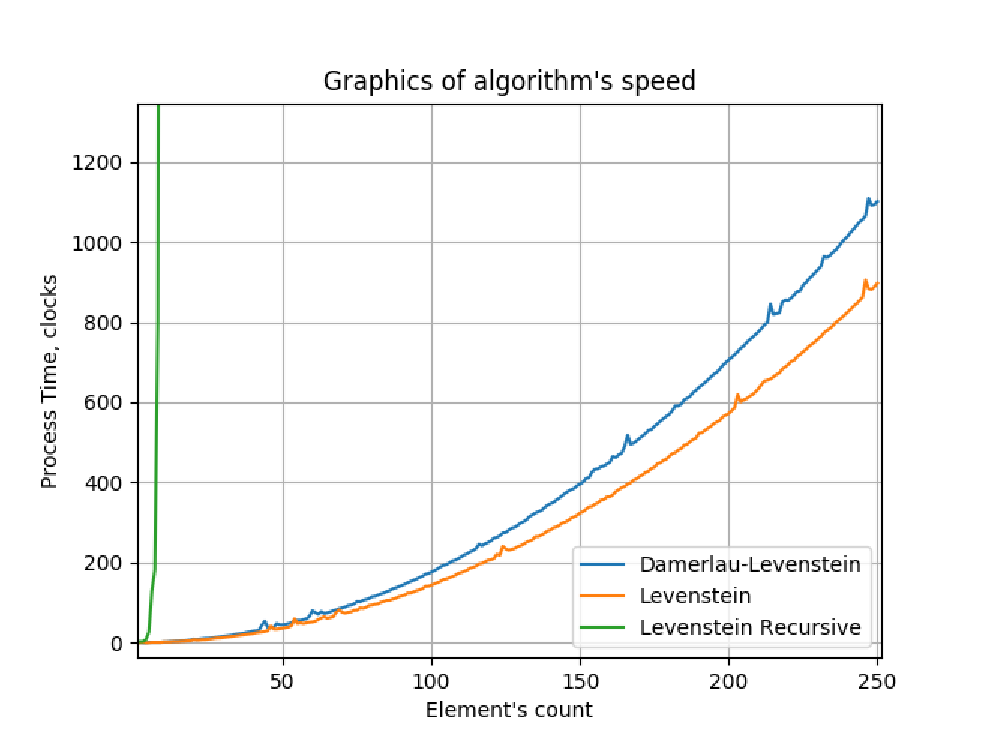
\includegraphics[scale=1]{graphics.eps}}
\caption{График зависимости времени работы алгоритмов от длин строк}
\label{images:graphics}
\end{figure}

\newpage
\subsection{Оценка затрачиваемой памяти}
1)Стандартный алгоритм Левенштейна (\hyperref[listings:listing1]{Листинг Кода 1}): \\
Используемый размер аппаратного стека = 60 байт (включая адрес возврата). \\
Используемый размер динамически выделенной памяти под матрицу: \\
$(l_1 + 1) * (l_2 + 1) * S$ байт, где \\
$l_1$ – длина первой строки (кол-во символов), \\
$l_2$ – длина второй строки, \\
$S$ – кол-во байт соответствующий выбранному типу данных. \\
Итого: Кол-во всей используемой памяти:
\begin{equation}
M = 60 + (l_1 + 1) * (l_2 + 1) * S
\end{equation}
2)Рекурсивный алгоритм Левенштейна (\hyperref[listings:listing2]{Листинг Кода 2}): \\
Используемый размер аппаратного стека для вызова одной функции = 46 байт, 40 байт для конечного вызова. \\
Для того, чтобы рекурсивная функция перестала вызывать саму себя, идет проверка на текущую длину строк. Если хотя бы одна строка имеет текущую длину 1, то находится
конечный результат (простейшее редакционное расстояние). \\
И тогда максимальный размер памяти (в аппаратном стеке), используемый во время
работы данной функции:\\
\begin{equation}
M = (l_1 - 1) * (l_2 - 1) * 46 + 40
\end{equation}
3)Алгоритм Дамерау-Левенштейна (\hyperref[listings:listing3]{Листинг Кода 3}): \\
Используемый размер аппаратного стека = 68 байт (включая адрес возврата). \\
Используемый размер динамически выделенной памяти под матрицу: \\
$(l_1 + 2) * (l_2 + 1) * S$ байт, где \\
$l_1$ – длина первой строки (кол-во символов), \\
$l_2$ – длина второй строки, \\
$S$ – кол-во байт соответствующий выбранному типу данных. \\
Итого: Кол-во всей используемой памяти:\\
\begin{equation}
M = 68 + (l_1 + 2) * (l_2 + 1) * S.
\end{equation}
В качестве используемого типа данных для матриц был выбран тип integer (4 байт). \\
Тогда сравнивая найденные значения размеров памяти для (4) и (5) получаем выражение: \\
\begin{equation}
21 * l_1 * l_2 - 25 * l_1 - 25 * l_2 < 7
\end{equation}
Это выражение истинно при значениях \{\{1, 1\}, \{1, 2\}, \{2, 2\}, \{2, 3\}\}, то есть только в этих случаях рекурсивный алгоритм будет эффективнее по памяти, чем стандартный. \\
Сравнивая 2) и 3) получаем: \\
\begin{equation}
21 * l_1 * l_2 - 25 * l_1 - 25 * l_2 < 7
\end{equation}
То есть данный случай можно рассматривать как эквивалентный предыдущему. \\

\newpage
\subsection{Вывод}

\newpage
\anonsection{ЗАКЛЮЧЕНИЕ}

В данной лабораторной работе был реализован алгоритм Левенштейна, позволяющий решать множество прикладных задач:автоматического исправления ошибок в слове, сравнения файлов, а в биоинформатике генов и хромосом. Проведено сравнение 3-х реализаций алгоритмов, выявлены их слабые места. Алгоритм с рекурсией является самым медленным, его стоит заменить базовым или модифицированным. Базовый и модифицированный сильно по скорости в данной реализации не различаются.



\newpage
\anonsection{СПИСОК ИСТОЧНИКОВ}
\begin{enumerate}
\item \label{sources:source1}Левенштейн В. И. Двоичные коды с исправлением выпадений, вставок и  замещений символов: Докл. Академий Наук СССР, 1965. С. 845–848. 
\item \label{sources:source2}D a m e r a u  F. A. Technique for Computer Detection and Correction of Spelling Errors // Communications of the ACM. 1964. Vol. 7. No. 3. P. 171–176.  
\item \label{sources:source3}Гасфилд. Строки, деревья и последовательности в алгоритмах. Информатика и вычислительная биология. Невский Диалект БВХ-Петербург, 2003.
\end{enumerate}

\end{document}
